\subsection{Broader exoplanet science}
\label{sec:broader_exoplanet_science}

\paragraph{Ephemeris times: analytic motivation}
\label{sec:ephemeris_timing_analytic}
If we want to know which extended mission scenario detects the most transiting planets, our yield statistics are directly applicable.
However, detection is a bare-minimum: we would also like to know when \tess planets transit long into the future.
For a planet with a ``stale'' ephemeris, follow up observations are more than just inconvenient.
Freshening ephemerides very probably will be a requirement before devoting significant observational resources like \jwst to a transiting planet.
Also, if the ephemeris gets very stale, we know that the star is transited but have essentially no idea when. 
For RV follow-up, a stale transit ephemeris will add uncertainty (or systematic bias) to the planetary mass estimate, because especially for low-mass planets, the predicted transit times are usually an important constraint of the orbital fit to the RVs.

Consider then the problem of estimating $\sigma_{t_c}(T_x)$, the uncertainty of the mid-transit time $\sigma_{t_c}$ for a given planet at some time $T_x$ following its last-observed transit. 
We begin analytically: assume that the planet has $N_\mathrm{tra}=2$ observed transits, spaced an orbital period $P=14$ days apart. Because that period is one half the nominal \tess dwell time of a given pointing, it represents the shortest period for which typically $N_\mathrm{tra}=2$, and as such the worst-case scenario for predicting the times of future transits, amongst cases with $N_\mathrm{tra}>1$.
Given two mid-transit times, each measured with the time's uncertainty $\sigma_0$, separated by $P$, the uncertainty of a future mid-transit time can be derived by standard least-squares fitting and propagation of errors (\textit{e.g.}~\citet{lyons_practical_1991}, Equation 2.18):
\begin{equation}
\sigma_{t_c}(T_x) = \sigma_0 \sqrt{1 + 2 T_x / P + 2 (T_x / P)^2 }
\end{equation}
Note that for observing future transits, $E \equiv T_x / P$ is an integer, and the above equation can be re-expressed:
\begin{equation}
\sigma_{t_c}(E) = \sigma_0 \sqrt{1 + 2 E + 2 E^2 },
\end{equation}
which is bounded by the simpler approximation: 
\begin{equation}
\sigma_{t_c}(E) \lesssim \sigma_0 \left(1+\sqrt{2} E\right), 
\end{equation}
which is exact at $E=0$, has a maximum 8\% fractional error at $E=1$, and becomes increasingly accurate as $E$ increases. By $E=20$, the fractional error of the latter approximation is less than 1\%.

For $T_x = 2$ years and $P = 2$ weeks, then $E \approx 50$, so $\sigma_{t_c}\approx 75\sigma_0$. 
At 2-minute cadence, a typical value for the per-transit timing uncertainty is $\sigma_0 = 4$ minutes, and the predicted uncertainty on its mid-transit time is 5 hours two years later or 10 hours four years later. This leads to a simple rule of thumb: % my oom is 5 minutes. Peter's is 2 minutes. The analytics are 5 minutes. I'll take the analytics.
\begin{quotation}
	The uncertainty of mid-transit times in hours is twice the number of years after \tess observes $N_\mathrm{tra}=2$ transits, for a typical super-Earth detection.	
\end{quotation}
If the transits are observed only at 30-minute cadence, then uncertainty will be roughly 4 times greater: $\sigma_0 \sim 16$ minutes. 
This claim (``$4\times$ greater'') is based on Figure 9 of~\citep{price_transit_2014}, a plot of the effects of finite cadence on timing precision. % note that they're using kepler data here 
We compared the precisions of 2-min and 30-min cadences for their specific example of $P=10$ days and a dwell time of 1 month.

On the other hand, Fig.~\ref{fig:Ntra_hist_primary} shows that 7 in 8 of the planets detected by \tesss main mission will have $N_\mathrm{tra}>3$ and so their ephemerides should be better than the example derived analytically above.
Rather than generalize the analytic equations, we resort to numerical simulations in order to predict the uncertainties of mid-transit times for planets expected to be discovered by \tesss main mission.

\paragraph{Ephemeris times: numerics}
We start with the analytic form~\citet{price_transit_2014} derive for the per-transit uncertainty on the mid-transit time $\sigma_0$:
$$
\sigma_{0} = \frac{1}{Q} \sqrt{ \frac{\tau T}{2} } \left( 1 - \frac{t}{3\tau} \right)^{-1/2}
$$
when $\tau\geq t$ and 
\begin{equation}
\sigma_{0} = \frac{1}{Q} \sqrt{\frac{t T }{2}} \left( 1 - \frac{\tau}{3t} \right)^{-1/2}
\label{eq:price_rogers}
\end{equation}
when $t > \tau$,
where $Q$ is the SNR per transit, $t$ is the cadence, $T$ is the transit duration, and $\tau$ is the ingress (or egress) time.
We have all the later terms from our yield simulation, and show the resulting distribution of $\sigma_0$ in Fig.~\ref{fig:uncertainty_tc_hist}.
Indeed, our suggested $\sigma_0$ of about 4 minutes for postage stamps and 16 minutes for full frame images is reasonable, which is good because we computed the former from the $t\rightarrow0$ limit of Eq.~\ref{eq:price_rogers} originally derived by~\citet{carter_analytic_2008}.
\begin{figure}[!t]
	\centering
	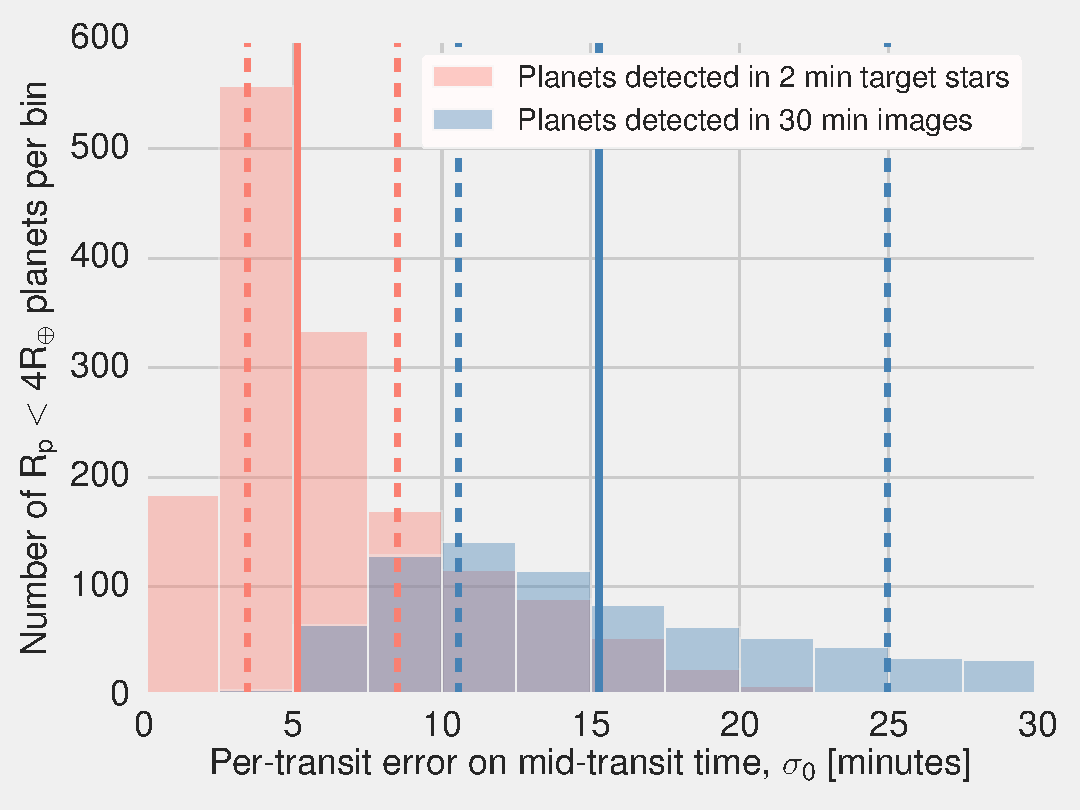
\includegraphics[scale=1.]{figures/mid_transit_time_vs_cadence.pdf}
	\caption{Uncertainty of mid-transit time on a single transit, $\sigma_{t_c}$, for all detected $R_p<4R_\oplus$ planets from the primary mission as computed from Eq.~\protect\ref{eq:price_rogers}.
	Solid lines are medians, dashed lines are 25$^\mathrm{th}$ and 75$^\mathrm{th}$ percentiles.
	}
	\label{fig:uncertainty_tc_hist}
\end{figure}
\begin{figure}[!t]
	\centering
	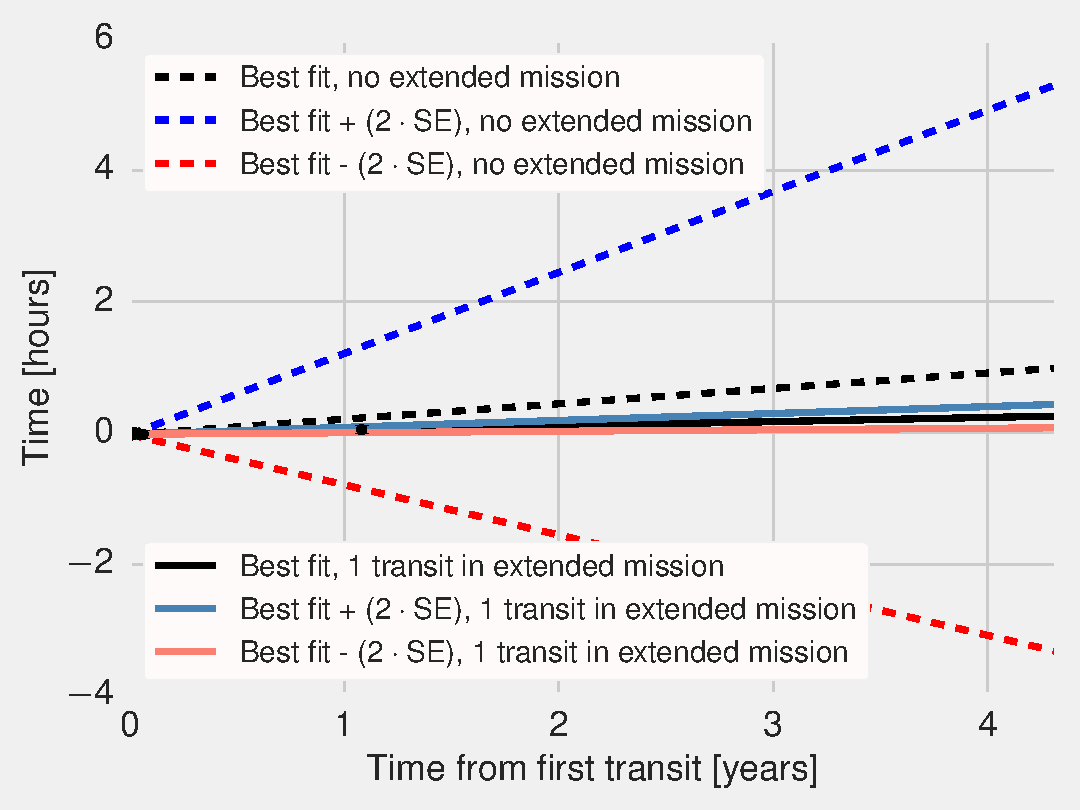
\includegraphics[scale=1.]{figures/lowering_uncertainty_on_midtransit_via_extra_point.pdf}
	\caption{	Observed mid-transit times (dots) and best fits to a linear ephemeris (lines).
		The dotted lines fit 4 data points from a nominal planet.
		`SE' is the standard error on the slope which multiplied by 1.96 (rounded to 2 in the legend) gives a 95\% confidence interval by subtracting blue and orange lines.
	}
	\label{fig:lowering_uncertainty_tc}
\end{figure}

Given the distributions on per-transit uncertainty of $t_c$, we then took an example planet with 4 transits.
We drew ``observed'' mid-transit times from a Gaussian with zero mean and standard deviation $\sigma_{0}$, and then ran a linear least squares regression. 
We then added just one data point 1 year after the final observed transit, and repeated the regression.
This produces a cartoon-plot, Fig.~\ref{fig:lowering_uncertainty_tc}, which confirms two expected points:
\begin{enumerate}
	\item Years after the initial discovery, the uncertainty of mid-transit time is of order hours.
	\item If we detect an additional transit 1 year after the final observed transit from the primary mission, the uncertainty on the mid-transit time decreases by an order of magnitude.
\end{enumerate}

\begin{figure*}[!t]
	\centering
	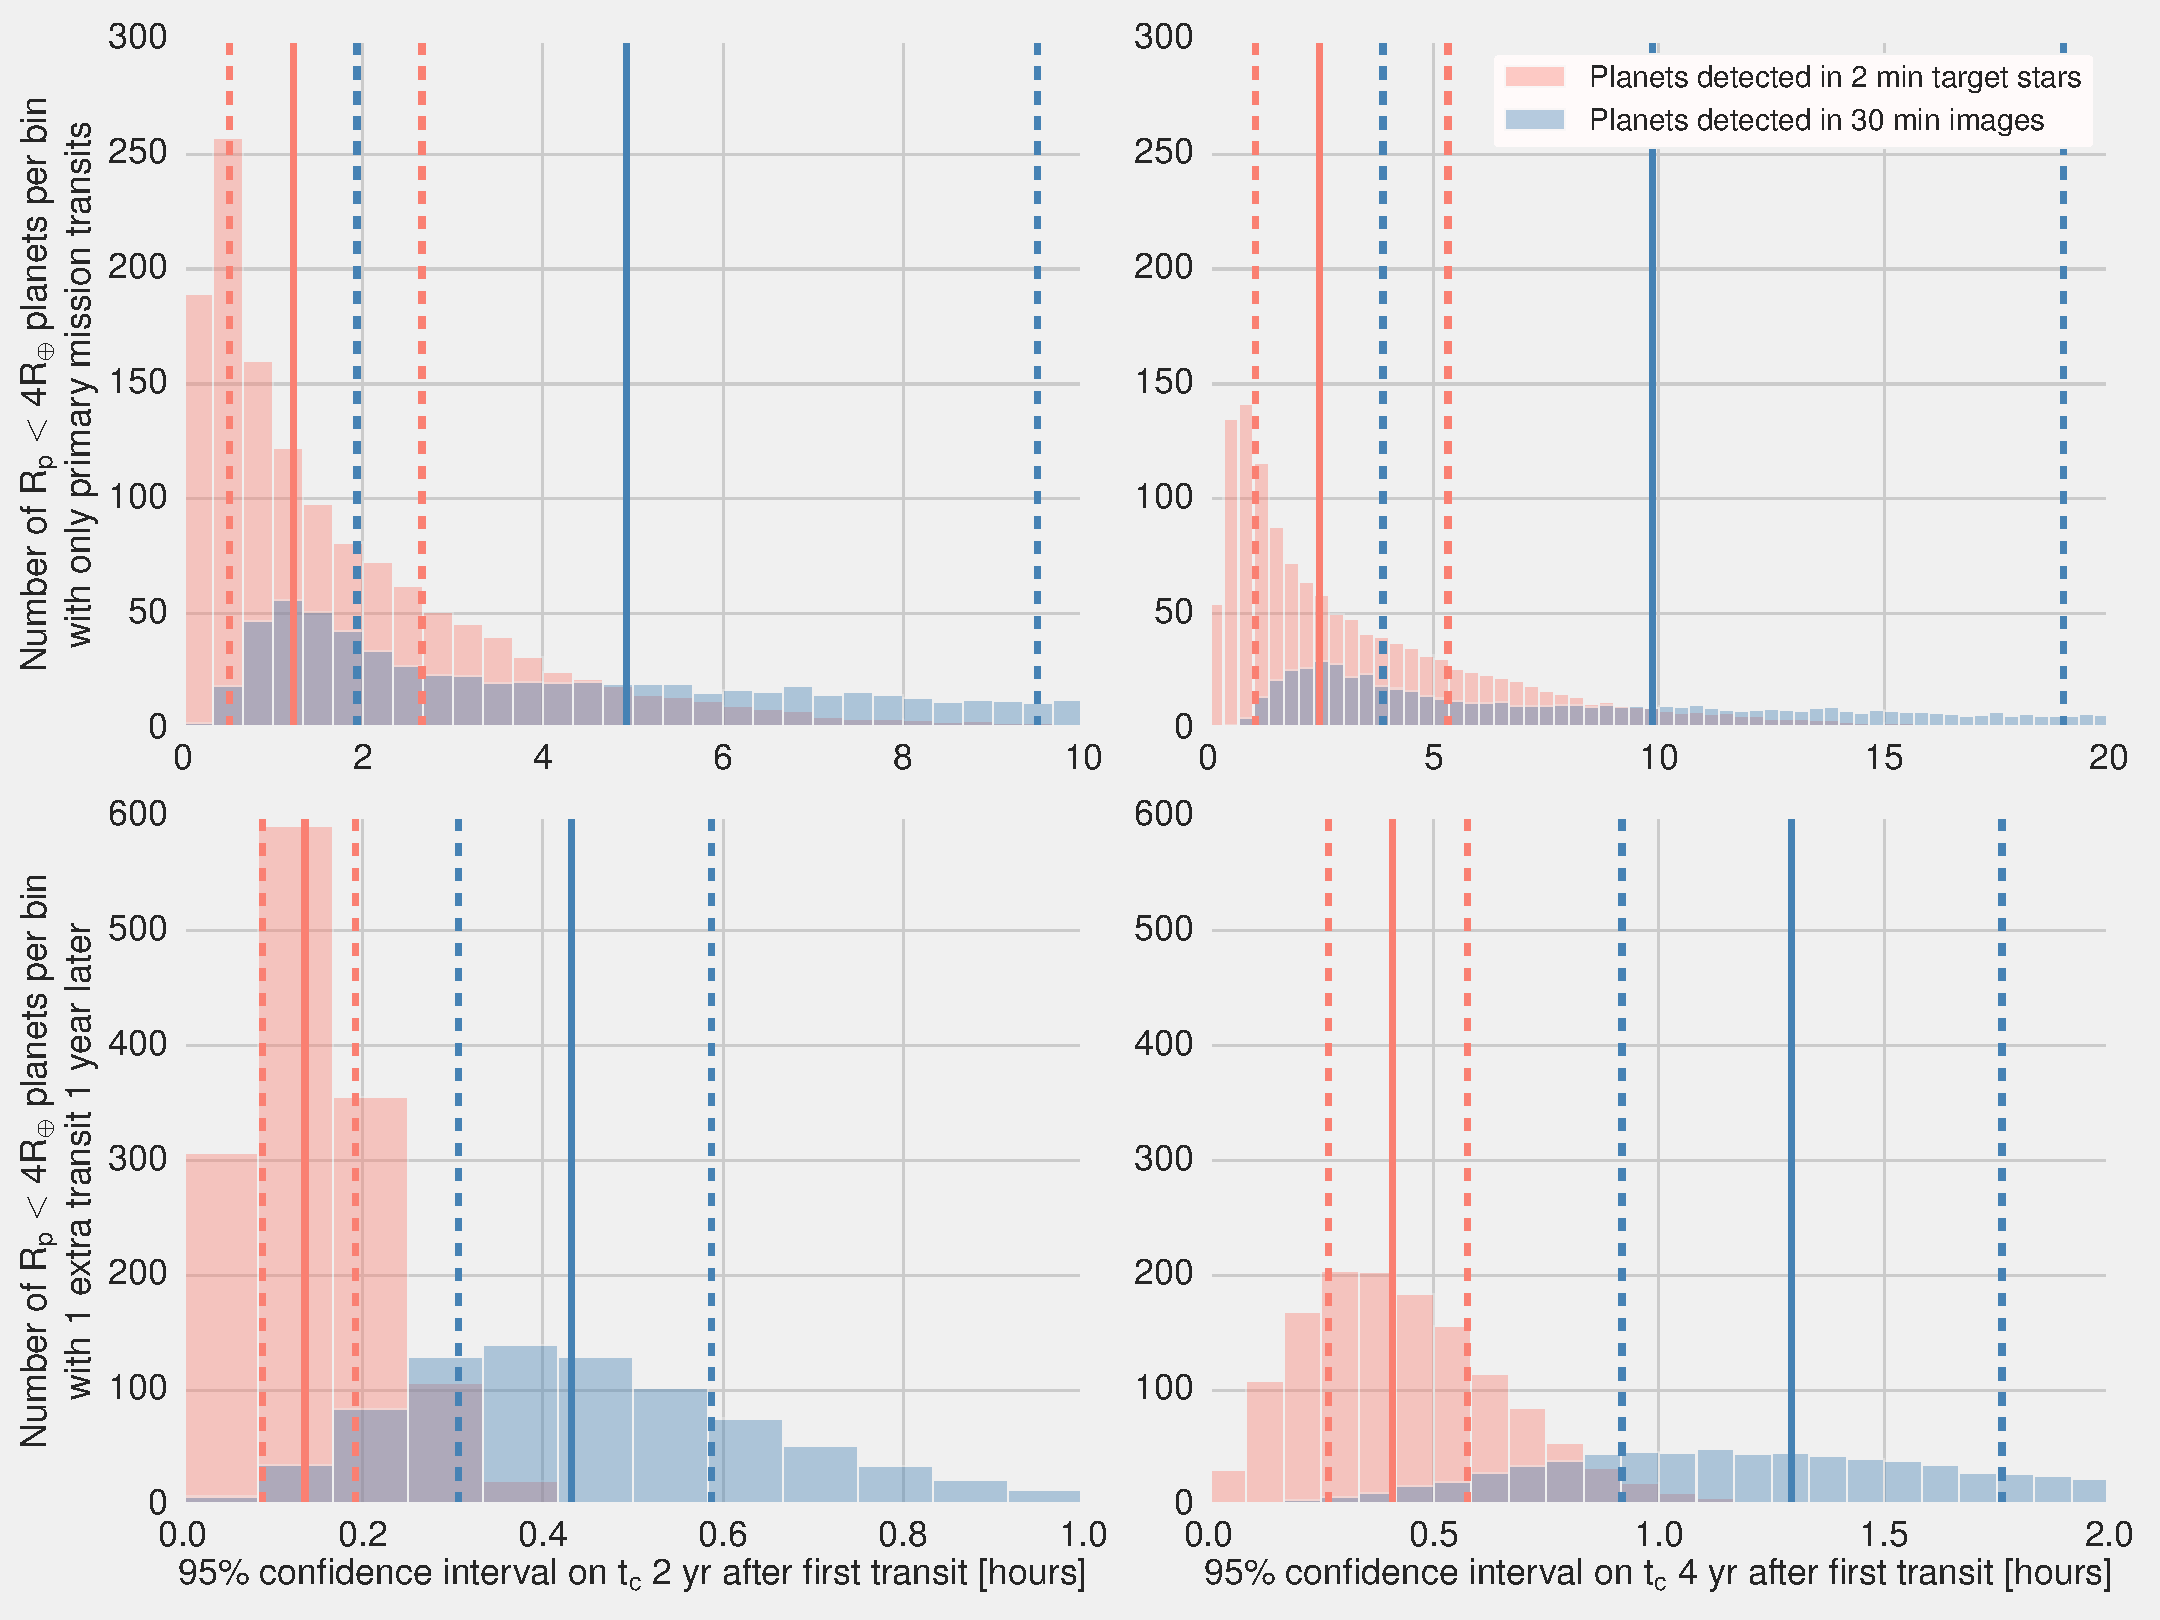
\includegraphics[scale=1.]{figures/confidence_interval_gets_better.pdf}
	\caption{\textit{Top row}: histogram of 95\% confidence intervals 2 (\textit{left}) and 4 (\textit{right}) years following the first detected transit in the primary mission.
	20 minute bins.
	\textit{Bottom row}: histogram of 95\% confidence intervals 2 (\textit{left}) and 4 (\textit{right}) years following the first detected transit in the primary mission, but with an additional data point added to the analog of Fig.~\protect\ref{fig:lowering_uncertainty_tc} one year after the transit in the initial time series (5 minute bins).
	Note that the top row's timescale is an order of magnitude more than the bottom row.
	Solid lines are medians, dashed lines are 25$^\mathrm{th}$ and 75$^\mathrm{th}$ percentiles.
	} %all in ephemeris_uncertainties.ipynb
	\label{fig:conf_interval_gets_better}
\end{figure*}
We proceed by repeating the above procedure for every planet, and evaluate typical 95\% confidence intervals (``uncertainties'', loosely) for $t_c$, at typical times after the first transits, for all of our detected planets.
Specifically, we take them at $T_x=2$ and $4$ years, and get Fig.~\ref{fig:conf_interval_gets_better}.
This figure confirms (top left panel) our analytic expectation that the uncertainty of mid-transit times in hours should be somewhat less than twice the number of years after \tess first observes the planet at 2-min cadence, since most such planets have $N_\mathrm{tra}\geq4$.
It also confirms our rough expectation that the uncertainty on FFI mid-transit times is roughly 4 times that of postage stamps, although the uncertainties on FFIs have a much more uniform tail.

More importantly, Fig.~\ref{fig:conf_interval_gets_better} emphasizes the importance of refining \tesss ephemerides: if we do not, the typical \tess planet will have many hours of uncertainty on its mid-transit time a few years following its detection.
If we do follow-up, we will know when the planet transits to $\lesssim1$ hour.
This argues strongly for an extended mission which, whether over 1 or 2 years, re-observes many if not all of the targets that \tess detects in its primary mission. 
The smallest-radius Earths and super-Earths may otherwise be irrecoverable.



\paragraph{Observe more transits over a long baseline to enable TTV measurements}
%Gravitational interactions between multiple bodies in a system with at least one transiting planet cause the planet's transit times to deviate from a linear ephemeris~\citep{agol_detecting_2005}.
Variations in transit times away from a linear ephemeris can be combined with planetary and orbital information derived from transits \textit{(a)} to confirm the planet-origin of transit signals and \textit{(b)} to determine the masses and system properties, for example mutual inclinations, of transiting and non-transiting planets~\citep{agol_detecting_2005}.

Our simulated dataset neglects orbital dynamics except to impose rule-of-thumb stability limits, assumes co-planarity between multiple planet systems, and assumes that multiple-planet system occurrence rates can be approximated as repeated draws from single-planet occurrence bins.
In short, it is insufficient to reliably predict TTV-detectability.
With that said, the best way to obtain useful TTV measurements is to observe as many high SNR transits as possible, over as long a baseline as possible.
Many TTV signals have timescales greater than a few years
%\todo[inline]{is there a nice formula? where does the $t^{5/2}$ scaling come from?}
and the information content in a TTV time series ideally scales as $t^{5/2}$~\citep{fabrycky_whitepaper_2013}.
Generally speaking then, the best extended mission scenario for measuring TTVs will include:
\begin{itemize}
	\item Long baseline observations of the same field, for instance one of \tesss continuous viewing zones.
	\item Observations of the \kepler field (for which measured transit times could resolve many TTV ambiguities from the 4-year dataset).
\end{itemize}
With these points in mind, \nhemi\ and \npole\ are likely the strongest scenarios for TTV detections over a single year's extended mission.

\begin{comment}
\textbf{Focus on compact multiple-planet systems}
\citet{muirhead_kepler-445_2015} estimate that $21^{+7}_{-5}\%$ of mid-M dwarfs host multiple planets with periods of less than 10 days.
\end{comment}



\paragraph{Targets beyond bright cool dwarf stars:}
\tesss main targets for the purpose of detecting small planets around bright stars are F-M dwarfs.
Observing other types of objects can enable broader exoplanet science.
For instance, we may wish to target:
\begin{itemize}
	\item open cluster members,
	\item known hosts of circumbinary planets,
	\item evolved stars (notably bright subgiants and red-giants for which it will be possible to detect asteroseismic oscillations, see below),
	\item all stars that are known to host transiting planets,
	\item all stars that are suspected to host \textit{any} planets (TOIs; KOIs from \kepler or \ktwo; candidates from \corot\!; candidates and confirmed planets from ground-based transit and RV surveys),
	\item white dwarfs,
	\item hot bright stars (OBA class),
	\item cool dwarf stars with spectral classes from late-M to mid-L,
	\item stars with well-measured properties from existing catalogs,
	%(for instance detailed abundance measurements, Hipparcos parallaxes, or very precise stellar parameters),

	\item eclipsing binaries and other multiple-star systems.
\end{itemize}
Some of these categories, notably asteroseismic targets, open cluster members, cool dwarfs, and circumbinary planets, have existing working groups dedicated to selecting targets and studying the resulting data once \tess begins its primary mission.
The \tess Target Star Selection team will incorporate target lists from these different working groups, while also incorporating many of the specific targets listed above\footnote{If the invested reader wishes to contribute to any of these lists, contact Joshua Pepper at \href{mailto:joshua.pepper@lehigh.edu}{joshua.pepper@lehigh.edu} or Keivan Stassun at \href{mailto:keivan.stassun@vanderbilt.edu}{keivan.stassun@vanderbilt.edu}} [Joshua Pepper, private communication].
\href{https://heasarc.gsfc.nasa.gov/docs/tess/}{Guest observer proposals} will likely also lead to allocation of pixels for many targets beyond bright F-M dwarf stars.

The relevance of all these objects to \tesss extended mission is that `observing time' (more precisely, data allocation) can be allotted differently between these targets in an extended mission than in the primary mission.
For instance, the benefits of obtaining precise stellar parameters and probing stellar physics via asteroseismology might merit a greater share of the data mass than is being proportioned for the primary mission.
The same could be argued for systems in which precise timing can greatly improve our ability to detect planets and characterize planetary systems.

We briefly highlight the cases for observing open clusters, circumbinary planets, asteroseismically-favorable targets, and stars with known or suspected planets below, and indicate which extended pointing scenarios we think will most benefit each observing program.

\begin{enumerate}
	\item \textit{Observing open clusters}.
	The main reasons to observe open clusters with \tess are (1) to discover planets in clusters (and then characterize them with other facilities) and (2) to perform stellar astrophysics relevant to exoplanets.
	Discovering planets in clusters will help determine their occurrence rate relative to field stars~\citep{meibom_same_2013}.
	This knowledge helps answer the question ``how well can small planets form and survive in dense clusters?''. 
	In terms of stellar astrophysics, an open cluster surveys also enables measurements of stellar rotation periods as a function of age (gyrochronology), which can constrain age-rotation-activity relations.
	Such a survey could also be used to identify eclipsing binaries in order to quantify their tidal evolution as a function of age.
	Soren Meibom is leading \tesss open cluster working group, which will construct lists of open cluster stars to be included in the \tess Candidate Target List.
	%It can also identify eclipsing binaries to quantify their stellar and tidal evolution.
	
	%The paragraph below based on the lists Meibom posted on the TESS wiki
	The majority of suitable open clusters with $V<16$ are near the galactic disk, and they are more common in the southern ecliptic hemisphere (with a south:north ratio of $\sim\!2:1$).
	While there are no known open clusters with $V<16$ at the north ecliptic pole's continuous viewing zone, there are a handful in that of the south ecliptic pole.
	Consequently, an extended mission scenario that observes the southern hemisphere, whether through the southern-conjugates of \nhemi\ and \npole, or through a scenario like \shemiAvoid, would be preferable for an open cluster survey.
	With that said, \npole\ would observe $\sim70$ open clusters with $V<16$, all within $42^\circ<\beta<68^\circ$.
	
	\item \textit{Circumbinary planets, circumprimary planets, and multiple star systems}.
	To date all $\sim$11 known circumbinary planets (CBPs) transit and are located in the \kepler field.
	Previous work has shown a statistical dearth of CBPs orbiting short-period ($P_\mathrm{bin} < 3$ day) eclipsing binaries~\citep{armstrong_abundance_2014,martin_planets_2014}, and formation requirements on such circumbinary planet systems are stronger than for planets orbiting EBs in which the EB has a relatively longer orbital period~\citep{martin_no_2015}.
	
	For order of magnitude purposes, consider two flavors of CBP detection from \tesss primary mission: those that are detected with $\ge3$ transits, and those with $\le 2$ transits.
	Assume that transiting CBPs will be mostly detected about eclipsing binaries (no CBPs to date are known to orbit a non-transiting eclipsing binary, although such objects likely exist in \keplers dataset \citep{martin_nontransiting_2014}).
	Given CBP orbital stability requirements, and the expectation that few CBPs will orbit $P_\mathrm{bin} < 3$ day eclipsing binaries, almost all of the $N_\mathrm{tra}\ge3$ CBP detections should happen in \tesss continuous viewing zones.
	Taking~\citetalias{Sullivan_2015}'s result that \tess will detect $\mathcal{O}(10^5)$ eclipsing binaries with $I<13$, and the fact that \tesss continuous viewing zones cover $2.2\%$ of the sky (908 deg$^2$), there will be roughly $2000$ EBs observed from one year over the primary mission.
	To date, \keplers Eclipsing Binary Working group has identified 2878 eclipsing and ellipsoidal binary systems of the 200,000 stars observed in \kepler\!'s 115 deg$^2$ field~\citep{kirk_keplerEB_2016}.
	This has led to $\sim$15 CBPs that are confirmed or in the process of being verified -- roughly a $0.5\%$ detection probability.
	Applying the same detection probability to \tesss CVZs, $\mathcal{O}(10)$ CBPs should be detected from 3 or more transits.
	
	For purposes of detecting CBPs from $\le 2$ transits, single-conjunction two-transit events will likely contribute to a major proportion of \tesss detections.
	Such events contain more information than single-star transits and can be used to make detections from a small number transits. 
	For instance, they enabled the confirmation of Kepler 1647b, the CBP with the longest known orbital period~\citep{kostov_kep1647b_2015}.
	Roughly 5 out of 1000 \kepler EBs with $P_\mathrm{bin}<30$ days had one-conjunction two-transit events [Haghighipour, private communication].
	Applying the same probability to \tess EBs means $\sim500$ \tess EBs will have these events.
	Perhaps 10\%-20\% will lead to CBP detections -- this means $\mathcal{O}(100)$ CBP detections from the \tess field outside of the CVZs.
	
	How will this affect the extended mission?
	The relative priority of these two different detection techniques -- robust CBP detections through $\ge 3$ transits in fields observed for a long time, vs. weak detections from $\le 2$ transits in fields observed for shorter durations -- merits further study.
	The former would advocate for a mission that maximizes the average observing time for all stars on a smaller sky area, for instance \npole.
	If this overlapped with the \kepler field, this would also enable \tess to detect transits of a subset of the \kepler CBPs.
	However the latter approach would argue for simply repeating the primary mission (\nhemi), or `event catching' single-conjunction two-transit events as in \hemis.
	
	Considering circum\textit{primary} planets, \tess should discover thousands of giant planets at orbital periods less than 10 days, predominantly in its full frame images, and with a heavy discovery bias towards the galactic disk (cf. Fig. 19 of ~\citetalias{Sullivan_2015}).
	Recent surveys have shown that roughly half of such hot Jupiter systems are expected to have stellar companions with semi-major axes between $50-2000\ \mathrm{AU}$~\citep{ngo_friends_2016}.
	The population of circumprimary planets that \tess will detect should be dominated by these systems.
	There should be a sufficiently large sample of these planets for follow-up imaging with adaptive optics to obtain CPP statistics, regardless of the extended mission.
	
	\item \textit{Asteroseismic targets}. See `Observing asteroseismic targets' paragraph in Sec.~\ref{par:asteroseismic_disc} below.
	
	
	\item \textit{Stars known or suspected to host transiting planets}. 
	If we know that the geometry of an exoplanetary system allows transits, the geometric bias against transit detection is removed.
	We should observe these targets \textit{(a)} to observe additional transits at precise times, enabling TTV searches, \textit{(b)} to obtain more precise photometry and thus refined parameters on known transiters, and \textit{(c)} in the case of ground-based detections, to observe companion transiting-planets that might not be detectable from the ground.
 	We discuss the prospects of \tess observing \kepler\!'s transiting planets in Sec.~\ref{par:TESS_as_followup}.
 	It will also be important to include the hosts of RV-detected planets in this sample. 
 	Although transit alignments are rare, combining transit and RV observables allows us to compute a planet's mean density, which is a necessary step towards detailed characterization. 
 	
 	For purposes of influencing an extended mission, the main bias in the currently known population of transiting planets is the \kepler field.
 	For an extended mission to follow up on the most currently-known transiting planets, it would be best target the northern ecliptic hemisphere, as in \npole\ or \nhemi.
	
	\item \textit{White dwarfs}.
	White dwarfs are scientifically interesting because of the window they offer into the long-term evolution of planetary systems.
	Their observational appeal for transit studies is that they have radii of $\mathcal{O}(R_\oplus)$, which means that transiting objects, whether planetary remnants (\textit{e.g.},~\citep{vanderburg_disintegrating_2015}), minor, or even major planets, produce large transit depths.
	However, the transit durations of major and minor planets are short ($T_\mathrm{dur} \sim R_\star / v_p$), and their transit probability is small ($\mathrm{prob}(\mathrm{tra}) \sim R_\star / a $).
	To date, no planets are known to transit white dwarfs (\citet{veras_postMS_2016} reviews the observational successes of the field along with this challenge).
	
	What this means for \tess is that a white dwarf survey would require short-cadence observations of many white dwarfs to overcome both the short transit durations and the low transit probability.
	While no group is currently advocating for this observing program, this may change by the time of an extended mission proposal.

\end{enumerate}

We do not discuss the observing cases for hot bright stars, late-M to mid-L dwarf stars, eclipsing binaries, or stars with well-measured properties.
% they can be made by say, GO observers

\begin{comment}
\paragraph{Microlensing survey}
Read relevant K2C9 papers. this is likely a bad idea (you can't get a good microlensing parallax like you could for K2C9)
\end{comment}